\scanpage{23}
are isomorphic to subgroups of the group of exterior automorphisms of $\mathrm{G}$) ?

In a different direction, it would 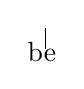
\begin{tikzpicture}[baseline=(be.base),x=1ex,y=1ex]\node[inner sep=0pt,anchor=base west] (be) at (0,0) {be};\draw[line width=.18pt] (1.54,1.05)--(1.54,2.55);\draw[line width=.35pt] (1.54,2.55)--(1.53,2.78);\end{tikzpicture}interesting to know more about the canonical morphism $\underline{\mathrm{g}}\handwritten{\longrightarrow}\underline{\mathrm{h}}/\mathrm{W}$, where $\underline{\mathrm{g}}$ is the Lie algebra of $\mathrm{G}$ and $\underline{\mathrm{h}}$ a Cartan subalgebra, and of the orbits of $\mathrm{G}$ on $\underline{\mathrm{g}}$, and the analoguous morphism of Steinberg $\mathrm{G}\handwritten{\longrightarrow}\mathrm{T}/\mathrm{W}$ and the orbits of $\mathrm{G}$ acting on itself. Do you know for instance exactly how varies the rank (= rang of the tangent map) of this \deleted{applic\unsure{at}i} map ? There are some reasons to believe that \deleted{this} for points of unipotent orbits of dimension \begin{tikzpicture}[baseline=(r.base),x=1ex,y=1ex]\node[inner sep=0pt,anchor=base west] (r) at (.4,0) {$\mathrm r-2$};\node[inner sep=0pt,anchor=base] at (0,1.40) {$\inserted{\mathrm n-}$};\draw[line width=.35pt] (-.90,1.65) .. controls (-1.05,.75) and (.03,.85) .. (.03,.25) -- (.03,-.45);\node[inner sep=0pt,anchor=center] at (-.20,-.16) {\unsure{\begin{tikzpicture}[x=1ex,y=1ex]\fill (0,0) circle (.035);\end{tikzpicture}}};\end{tikzpicture} (just 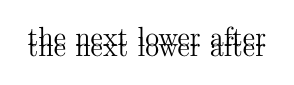
\begin{tikzpicture}[baseline=(live.base),x=1ex,y=1ex]\node[inner sep=0pt,anchor=base west] (live) at (0,0) {\inserted{the next lower after}};\node[inner sep=0pt,anchor=base west] at (0,.80) {\deleted{the next lower after}};\end{tikzpicture} the maximal dimension $\mathrm{n}-\mathrm{r}$), the rank is $\mathrm{r}-1$ in case all roots have same length (that is the corresponding diagrams $\mathrm{A}_{\unsure{\begin{tikzpicture}[baseline=(m.base),x=1ex,y=1ex]\node[inner sep=0pt,anchor=base] (m) at (0,0) {$\scriptstyle\mathrm r$};\node[inner sep=0pt,anchor=base] at (.08,-.06) {$\scriptstyle\mathrm n$};\end{tikzpicture}}},\mathrm{D}_{\unsure{\begin{tikzpicture}[baseline=(m.base),x=1ex,y=1ex]\node[inner sep=0pt,anchor=base] (m) at (0,0) {$\scriptstyle\mathrm r$};\node[inner sep=0pt,anchor=base] at (.08,-.06) {$\scriptstyle\mathrm n$};\end{tikzpicture}}},\mathrm{E}_{\handwritten{6}},\mathrm{E}_{\handwritten{7}},\mathrm{E}_{\handwritten{8}}$ are those corresponding to Klein singularities), and $\handwritten{<}\mathrm{r}-1$ in 
\begin{tikzpicture}[baseline=(other.base),x=1ex,y=1ex]\node[inner sep=0pt,anchor=base west] (other) at (0,0) {other};\node[inner sep=0pt,anchor=base west] at (-.48,1.25) {\inserted{\handwritten{all}}};\draw[line width=.22pt] (1.52,1.42) .. controls (1.38,.66) and (-.20,.70) .. (-.44,-.02);\end{tikzpicture} cases; in the first case, I would expect that there is just one orbit as stated, by the way, and maybe this property will be caracteristic of the ``homogene\deleted{\unsure{a|u}}ous'' case when all roots have same length. Also, what can be said of the dim\unsure{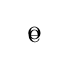
\begin{tikzpicture}[baseline=(m.base),x=1ex,y=1ex]\node[inner sep=0pt,anchor=base] (m) at (0,0) {e};\node[inner sep=0pt,anchor=base] at (.03,.24) {o};\end{tikzpicture}}nsion of the set of all Borel subgroups containing a given element $\mathrm{g}\handwritten{\in}\mathrm{G}$, resp. whose Lie algebra contains a given element $\mathrm{x}\handwritten{\in}\underline{\mathrm{g}}$ ? If $2\mathrm{N}=\mathrm{n}-\mathrm{r}$ is the number of roots and if the dimension of the orbit of the given element is $2\mathrm{N}-2\mathrm{i}$, I would expect the dimension of the previous variety to be equal to $\mathrm{i}$; the inequality $\handwritten{\leqslant}\mathrm{i}$ would imply, by generalizing a depth argument of Br\unsure{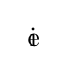
\begin{tikzpicture}[baseline=(m.base),x=1ex,y=1ex]\node[inner sep=0pt,anchor=base] (m) at (0,0) {i};\node[inner sep=0pt,anchor=base] at (.03,-.03) {e};\end{tikzpicture}}\unsure{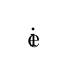
\begin{tikzpicture}[baseline=(m.base),x=1ex,y=1ex]\node[inner sep=0pt,anchor=base] (m) at (0,0) {e};\node[inner sep=0pt,anchor=base] at (-.02,.09) {i};\end{tikzpicture}}skorn, that the singularities of the fibers of your map $\underline{\mathrm{g}}\handwritten{\longrightarrow}\underline{\mathrm{h}}/\mathrm{W}$ (resp. Steinberg's $\mathrm{G}\handwritten{\longrightarrow}\mathrm{T}/\mathrm{W}$ in case $\mathrm{G}$ is simply connected instead of adjoint) are ``rational'', i.e. i\unsure{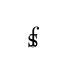
\begin{tikzpicture}[baseline=(m.base),x=1ex,y=1ex]\node[inner sep=0pt,anchor=base] (m) at (0,0) {f};\node[inner sep=0pt,anchor=base] at (-.03,-.02) {s};\end{tikzpicture}} $\mathrm{F}$ is such a fiber and $\mathrm{F}'\overset{\mathrm{f}}{\handwritten{\longrightarrow}}\mathrm{F}$ a resolution of singularities of $\mathrm{F}$, t\unsure{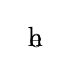
\begin{tikzpicture}[baseline=(m.base),x=1ex,y=1ex]\node[inner sep=0pt,anchor=base] (m) at (0,0) {h};\node[inner sep=0pt,anchor=base] at (.04,-.04) {e};\end{tikzpicture}}\unsure{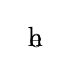
\begin{tikzpicture}[baseline=(m.base),x=1ex,y=1ex]\node[inner sep=0pt,anchor=base] (m) at (0,0) {e};\node[inner sep=0pt,anchor=base] at (-.03,.05) {h};\end{tikzpicture}}n $\mathrm{R}^{\mathrm{i}}\mathrm{f}_{\handwritten{*}}(\underline{\mathrm{O}}_{\mathrm{F}'}^{\deleted{\unsure{*|\mathrm{t}}}})=0$ for $\mathrm{i}\handwritten{>}0$. Maybe the ans\unsure{
\begin{tikzpicture}[baseline=(m.base),x=1ex,y=1ex]\node[inner sep=0pt,anchor=base] (m) at (0,0) {w};\node[inner sep=0pt,anchor=base] at (.02,-.03) {u};\end{tikzpicture}}\unsure{\begin{tikzpicture}[baseline=(e.base),x=1ex,y=1ex]\node[inner sep=0pt,anchor=base west] (e) at (0,0) {e};\draw[line width=.24pt] (.03,.90)--(.03,1.47);\end{tikzpicture}}r \deleted{\unsure{ot|to}}\handwritten{to} most of the questions I am asking are well known and I am just ignorant; for some of them, it would indeed be scandalous that the experts do not know the answer ! In any case, I would be grateful for any comment you would have on any of my questions.

\noindent\hspace*{.08\linewidth}Sincerely yours\\
\hspace*{.62\linewidth}\handwritten{A\,G\unsure{rothendieck}}\\
% The short vertical trace is above the e of beinteresting, not a supplied space.
% Raised n- is letter-for-letter certain; its typed-looking serifs leave medium uncertain (typed preferred).
% The separate low point beside the n- insertion leader is preserved without assigning punctuation.
% The A/D, dimension, Brieskorn, if and then superpositions do not establish strike order.
% The e in answer has an extra left upright; its function is uncertain.
% Signature initial A and G are legible; the compressed remainder remains locally doubtful.
% A disconnected interrupted vertical trace in the lower blank is reproduced below.
% Whether this lower trace is ink or a surface mark is unresolved.
\figure{\hspace*{.60\linewidth}\unsure{\begin{tikzpicture}[x=1cm,y=1cm]
\draw[line width=.24pt] (.015,.90)--(.013,.79);
\draw[line width=.24pt] (.011,.75)--(.009,.61);
\draw[line width=.24pt] (.008,.57)--(.005,.34);
\draw[line width=.24pt] (.005,.30)--(0,.10);
\end{tikzpicture}}}
% archive sheet number: 22
